% -----------------------------------------------------------------------------
% Description: Quantitative Results (Table 6, 7, 8 from paper)
% -----------------------------------------------------------------------------

\begin{frame}{Quantitative Performance Analysis}
    \centering
    \vspace{-0.2cm}

    % --- Insight Box ---
    \begin{beamercolorbox}[sep=5pt, center, rounded=true, shadow=false, bg=blue!5]{insight}
        \small \textbf{Key Insight:} Dual-Model Fusion achieves the best balance, significantly boosting \textbf{Sensitivity} (+12.5\%) compared to the baseline.
    \end{beamercolorbox}

    \vspace{0.4cm}

    % --- Comparison Table ---
    \renewcommand{\arraystretch}{1.4}
    \setlength{\tabcolsep}{10pt}
    \resizebox{0.95\textwidth}{!}{%
    \begin{tabular}{lcccc}
        \toprule
        \textbf{Model Strategy} & \textbf{Accuracy} & \textbf{Precision} & \textbf{Sensitivity} & \textbf{F1-Score} \\
        \midrule

        % Base VGG16 (Grayed out slightly as baseline)
        \color{gray} Base VGG16 ($L_1$) & \color{gray} 83.54\% & \color{gray} 90.91\% & \color{gray} 75.00\% & \color{gray} 82.19\% \\

        % Tuned VGG16
        Tuned VGG16 ($L_2$) & 87.34\% & \textbf{94.12\%} & 80.00\% & 86.49\% \\

        \midrule

        % Fused Model (Highlighted Row)
        \rowcolor{DeepBlue!10}
        \textbf{Fused VGG16 ($L_1 \lor L_2$)} & \textbf{89.87\%} & 92.11\% & \textbf{\textcolor{red}{87.50\%}} & \textbf{89.74\%} \\
        \bottomrule
    \end{tabular}
    }

    \vspace{0.5cm}

    % --- Visual Metric Improvement (Mini Bar Chart using TikZ) ---
    \begin{columns}
        \begin{column}{0.3\textwidth} \raggedleft \footnotesize \textbf{Sensitivity Gain:} \end{column}
        \begin{column}{0.6\textwidth}
            \begin{tikzpicture}
                % Base
                \fill[gray!50] (0,0) rectangle (3.0, 0.4) node[right, black] {75.0\%};
                % Tuned
                \fill[DeepBlue!50] (0,-0.6) rectangle (3.2, -0.2) node[right, black] {80.0\%};
                % Fused
                \fill[red!70] (0,-1.2) rectangle (3.5, -0.8) node[right, black] {\textbf{87.5\%}};

                % Y-Axis Line
                \draw[thick] (0,-1.4) -- (0,0.6);
            \end{tikzpicture}
        \end{column}
    \end{columns}
\end{frame}



% -----------------------------------------------------------------------------
% File: sections/04_results/2_confusion_matrix.tex
% Description: Confusion Matrix Visualization (Focus on FN Reduction)
% -----------------------------------------------------------------------------

\begin{frame}{Clinical Impact: Reducing Missed Diagnoses}
    \centering

    \begin{columns}
        % --- LEFT: BASE MODEL ---
        \begin{column}{0.45\textwidth}
            \centering
            \textbf{Base VGG16} \\
            \vspace{0.2cm}
            \resizebox{0.8\textwidth}{!}{%
            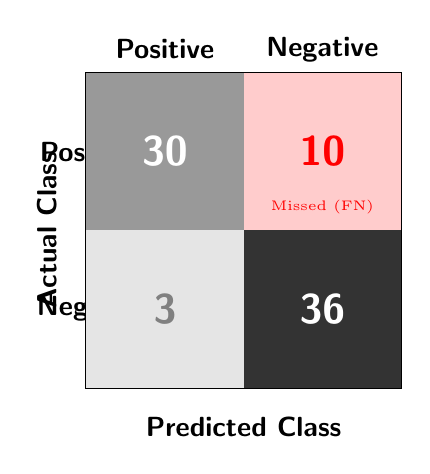
\begin{tikzpicture}[font=\sffamily\bfseries]
                % Grid
                \draw[thick] (0,0) rectangle (4,4);
                \draw[thick] (2,0) -- (2,4);
                \draw[thick] (0,2) -- (4,2);

                % Labels
                \node[rotate=90] at (-0.5, 2) {Actual Class};
                \node at (2, -0.5) {Predicted Class};
                \node at (1, 4.3) {Positive}; \node at (3, 4.3) {Negative};
                \node at (-0.3, 3) {Pos}; \node at (-0.3, 1) {Neg};

                % Data (From User Image Fig 3: TP 30, FN 10)
                % TP (Top Left)
                \fill[gray!80] (0,2) rectangle (2,4);
                \node[white, scale=1.5] at (1,3) {30};

                % FN (Top Right) - THE PROBLEM
                \fill[red!20] (2,2) rectangle (4,4);
                \node[red, scale=1.5] at (3,3) {10}; % High Miss Rate
                \node[red, font=\tiny] at (3,2.3) {Missed (FN)};

                % FP (Bottom Left)
                \fill[gray!20] (0,0) rectangle (2,2);
                \node[gray, scale=1.5] at (1,1) {3};

                % TN (Bottom Right)
                \fill[black!80] (2,0) rectangle (4,2);
                \node[white, scale=1.5] at (3,1) {36};
            \end{tikzpicture}
            }
        \end{column}

        % Arrow between matrices
        \begin{column}{0.1\textwidth}
            \centering
            \Huge $\Rightarrow$
        \end{column}

        % --- RIGHT: FUSED MODEL ---
        \begin{column}{0.45\textwidth}
            \centering
            \textbf{\textcolor{DeepBlue}{Fused VGG16}} \\
            \vspace{0.2cm}
            \resizebox{0.8\textwidth}{!}{%
            \begin{tikzpicture}[font=\sffamily\bfseries]
                % Grid
                \draw[thick, DeepBlue] (0,0) rectangle (4,4);
                \draw[thick, DeepBlue] (2,0) -- (2,4);
                \draw[thick, DeepBlue] (0,2) -- (4,2);

                % Data (From User Image Fig 5: TP 35, FN 5)
                % TP
                \fill[DeepBlue!80] (0,2) rectangle (2,4);
                \node[white, scale=1.5] at (1,3) {35};

                % FN - THE IMPROVEMENT
                \fill[green!20] (2,2) rectangle (4,4);
                \node[green!60!black, scale=1.5] at (3,3) {5}; % Reduced!
                \node[green!60!black, font=\tiny] at (3,2.3) {\textbf{-50\% Misses}};

                % FP
                \fill[gray!20] (0,0) rectangle (2,2);
                \node[gray, scale=1.5] at (1,1) {3};

                % TN
                \fill[black!80] (2,0) rectangle (4,2);
                \node[white, scale=1.5] at (3,1) {36};
            \end{tikzpicture}
            }
        \end{column}
    \end{columns}

    \vspace{0.5cm}
    \begin{beamercolorbox}[sep=4pt, center, rounded=true, bg=green!10]{conclusion}
        \small
        The Fusion Strategy successfully \textbf{rescued 5 Alzheimer's patients} (TP: $30 \to 35$) who were missed by the Base model.
    \end{beamercolorbox}
\end{frame}